\chapter{If-Conversion \Author{C. Bruel}}\label{chap:if_conversion}
\inputprogress
\label{chap:if_conv}
\graphicspath{{img/}{if_conversion/img/}{part4/if_conversion/img/}}

\newcommand\cond{~?~}
\newcommand{\annotation}[1]{%
  \marginpar{\small\itshape\color{red}#1}}

%\setcounter{tocdepth}{3} 
%\tableofcontents

\section{Introduction}

The instruction throughput can be improved by increasing the IPC (number of instructions per cycle). This can be achieved either by increasing the pipeline depth, or by increasing the number of instructions that are executed simultaneously.

In order to exploit this ILP, VLIW (Very Large Instruction World) or EPIC (Explicitly Parallel Architectures) make the parallelism visible into the ISA (Instruction Set Architecture), relying on the static scheduler to organize the compiler output so that multiple instructions can be issued in each cycle.

Conditional branches introduce control dependencies between instructions. An instruction is control dependent on a preceding instruction if the preceding instruction determines the execution of the one. These conditional branches act as a bottleneck for exposing parallelism.

Removing branches improves performance in several ways: by removing the misprediction penalty, the instruction fetch throughput is increased and the instruction cache miss penalty reduced. Enlarging the size of the basic blocks allows earlier execution of long latency operations and merge of multiple control flow paths into a single flow of execution, that profit to scheduling frameworks, such as VLIW scheduling, hyperblock scheduling, modulo scheduling. Another benefit is that classical local transformations are now unleashed.

If-conversion is the process of transforming a region of control dependent instructions into an equivalent sequence of instructions, where conditional branches have been removed. 

If-conversion is a global optimization, aiming at efficient CFG region selection and reconstruction, and a local problem, to best select and emit the new conditional and predicate setting operations.
We propose an if-conversion algorithm under SSA, that transforms a CFG region in SSA form to produce an if-converted SSA representation using control speculation.
Then we describe how this framework is extended to use predicated instructions, using the $\psi$-SSA form presented in chapter~\ref{chap:psi_ssa}.

Consider the simple example \ref{fig:example1}, that represents the execution of an if-then-else statement on a 4-issue processor. Branches are highly biased, so the basic blocks can be reordered to favor the critical path. Even with this optimistic case, the schedule height is still 6 cycles (assuming that all instructions have a one cycle latency), with a maximal schedule height of 7 instructions. 

\begin{figure}
\footnotesize
  \subfloat[Control Flow] {
    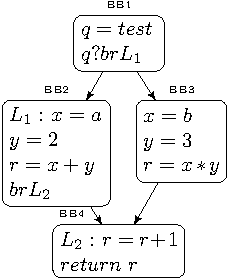
\includegraphics{specul}
    \label{fig:orig}}

  \subfloat[with basic block ordering] {
     \begin{tabular}[t]{lllll}
      & ALU1 & ALU2 & ALU3 & ALU 4 \\
\hline
      & $q = test$         &   -     &   -   & - \\
      & $q \cond br$ $L_1$ & -       & - & - \\
      & $x = 2$            & $y = 3$ & - & - \\
      & $r = x * y$ & - & - & - \\
$L_2$ & $r = r + 1$ & - & - & - \\
      & $return$ $r$ & - & - & - \\
$L_1$ & $x = a$ & $y = 2$ & - & - \\
      & $r = x + y$ & - & - & - \\
      & $br$ $L_2$ & - & - & - \\
     \end{tabular}}
\vspace{1cm}
  \subfloat[After if-conversion] {
     \begin{tabular}[t]{lllll}
      & ALU1 & ALU2 & ALU3 & ALU 4 \\
\hline
      & $q = test$ & - & - & - \\
      & $x_1 = 2$ & $y_1 = 3$ & $x_2 = a$ & $y_2 = 2$ \\
      & $r_1 = x_1 * y_1$ & $r_2 = x_2 + y_2$ & - & - \\
      & $r = q \cond r_1 : r_2$ & - & - & - \\
      & $return$ $r$ & - & - & - \\
      & & & & \\     
      & & & & \\     
      & & & & \\     
      & & & & \\     
     \end{tabular}}
\caption{Static schedule of a simple region on a 4 issue processor}
\label{fig:example1}
\end{figure}

After if-conversion the execution path is reduced to 5 cycles, regardless of the tests outcomes.

From this introductory example, we can observe that the transformation implies:

\begin{itemize}
\item The merge of execution paths into a single execution path, implying a  better exploitation of available resources.  
\item The reduction of the schedule length, because instructions can be speculated before the branch.
\item That the variables need to be renamed, production of new data dependencies.
\item The introduction of a \textit{merge} pseudo operation.
\end{itemize}

% \annotation{Reference join sets; phi-congruence already here?}
Thanks to SSA, the merging point is already materialized into the original control flow by the $\phi$ pseudo operation and register renaming is a basic property of SSA. Given those similarities between SSA and the if-conversion requirements, the transformation to generate if-converted code seems natural. We describe here the framework to use those properties on more complex regions.

\subsection{Architectural requirements}

The \textit{merge} pseudo operations needs to be mapped to a conditional form of execution on the target's architecture. \ref{fig:pred} shows different models of conditional execution that the algorithm can use, thanks to:

\begin{itemize}
\item Speculative execution by mean of conditional moves, using temporary registers.
\item Predicated execution by mean of architectural feature that allows an instruction to be executed conditionally by mean of a predicate operand.
\item A partially predication model can be used to predicate only the subset of the ISA that are not easily speculable, usually memory operations. Other instructions are speculated.
\end{itemize}

\begin{figure}
\footnotesize
\begin{minipage}[t]{3cm}
\mbox{fully predicated} \\
$p \cond x = a + b $ \\
$\overline{p} \cond x = 0 $ \\
\end{minipage} 
\begin{minipage}[t]{3cm}
\mbox{select} \\
$t = a + b $ \\
$x= p \cond t : 0 $ \\
\end{minipage}
\begin{minipage}[t]{3cm}
\mbox{cmov} \\
$t = a + b $ \\
$x = 0 $ \\
$x = cmov p,t$ \\
\end{minipage}
\caption{Conditional execution using different models}
\label{fig:pred}
\end{figure}

To be speculated, an instruction must not potentially create any side effects, or hazards. For instance a memory load must not trap (cache misses can also be considered for performance). This prevents the conditional execution by means of speculation of memory access for which the address is valid only on the selected path. Other reasons are may-alias problems during the memory instructions layout. Memory operations are therefore a major impediment to if-conversion. This is regrettable, because as long latency operations, speculative load can be very effective to fetch data earlier in the instruction stream, reducing stalls. Modern architectures provide architectural supports to dismiss invalid address exceptions. Examples are the $ldw.d$ dismissible load operation of the $ST231$ or $multiflow$ processors or the $IA64$ speculative loads. Note that $IA64$ provides both speculative and predicate loads.

\begin{figure}
\begin{minipage}[t]{4cm}
\mbox{IA64 speculative load} \\
$t = ldw.s(addr) $ \\
$jump$ $l_1:$ \\
$check.s\:t$ \\
$x = t$ \\
\end{minipage}
\begin{minipage}[t]{4cm}
\mbox{Multiflow dismissible load} \\
$t = ldw.d(addr) $ \\
$x = select\: \cond t : x $ \\
\end{minipage}

\begin{minipage}[t]{4cm}
\mbox{base store hoisting} \\
$x=select\:p \cond addr : dummy $ \\
$stw (x, value) $ \\
\end{minipage}
\begin{minipage}[t]{4cm}
\mbox{index store hoisting} \\
$index=select\:p \cond i : j $ \\
$stw (x[index], value) $ \\
\end{minipage}
\label{fig:spec}
\caption{Example of speculated memory operations}
\end{figure}

Stores can be performed by speculating the address value, and forcing it to be a dummy valid address in the case of not taken path. Naturally store hoisting can only be done if there is no aliasing conflict between different memory operations merged into a single execution path. 

\section{Global Analysis and Transformations}

The traditional approach to perform if-conversion in SSA is to apply a classical if-conversion algorithm, such as Fang or RK, on a conventional SSA representation. Assuming that all instructions are predicated, an additional pass is required during instruction selection to emit speculative instructions when predicated variant is not available. Another pass is usually applied for predicate promotion, based on predicate dependence graph, that allows to break data dependencies between a predicate setting operation and its use.
During the if-conversion process, instructions that merged into the deleted $\phi$ operations are expressed into $\psi$ operations, merging different values from their $\psi-congruence$ class. 

To illustrate the differences between a traditional framework and a native SSA framework, we first start to describe a well known RK algorithm proposed by Park and Schlansker on the nested tests from figure In \ref{fig:nested1}. We will then describe in detail the SSA based approach.

Standard if-conversion techniques address the problem in the following order: First, identify the region to if-converted. An execution trace is selected based on profiling information to isolate the region. Then allocate boolean variables to the basic blocks, on the identified region. Then perform predicate initialization placement, instruction emissions and CFG restructuration into the final if-converted regions.

The RK algorithm starts by computing the Control Dependence Graph. It is necessary to associate each basic blocks a guard condition, and to associate each guard the set of basic blocks that need to set it. The algorithm creates a new guard, eventually initialized to false, for each condition. \ref{fig:nested2} shows the sub-region with new conditions initialized, and \ref{fig:RK} the RK mappings.

\begin{figure}
\centering
  \subfloat[Nested test] {
    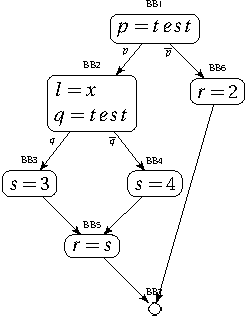
\includegraphics[scale=0.8]{nested1}
    \label{fig:nested1}}
  \subfloat[Predicate Assignments] {
    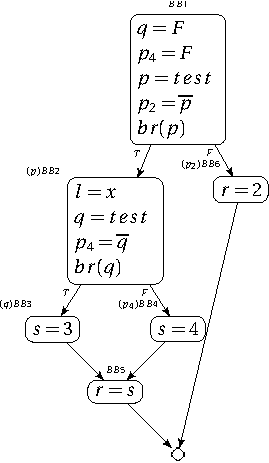
\includegraphics[scale=0.8]{nested1_rk}
    \label{fig:nested2}}
  \subfloat[After Instruction layout] {
    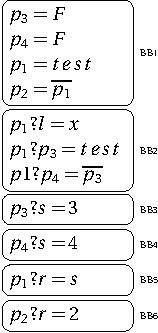
\includegraphics[scale=0.8]{nested1_rk2}
    \label{fig:nested}}
\caption{Classical support for partial predication}
\label{fig:trad_part_pred}
\end{figure}

\begin{figure}
\footnotesize
  \subfloat[R mapping] {
     \begin{tabular}[t]{|l|cccccc|}
\hline
      Basic Block & BB1 & BB2 & BB3 & BB4 & BB5 & BB6  \\
\hline
      Guard       &  T  &  p   & q  & p4  &  p  &  p2 \\
\hline
     \end{tabular}}
  \subfloat[K mapping] {
     \begin{tabular}[t]{|l|cccc|}
\hline
      Guard          & p & q & p4  & p2  \\
\hline
      Basic Block    & 1 & 2,-0 & -2,-0 & -1 \\
\hline
     \end{tabular}}
\caption{Output from RK algorithm}
\label{fig:RK}
\end{figure}

By the end, the algorithm merge the basic blocks, using the predicates and the conditionalized instructions, and removes the instruction branches. \ref{fig:nested}. 

This approach assumes that all instructions can be predicated, and in particular the predicate setting operations (test) which need to be conditionalized. Without predicate support for comparison instructions, logical operations must be used to merge condition setting operations. For instance, in the given example, the initialization sequence $p_1 ? p_3=test$ needs to be rewritten as $t=test; p_1=p_3 \& t$. An algorithm based on speculative transformations, necessary to handle efficiently partially predicated architectures, is then penalized by this approach, since a rewritten pass is needed to convert a conditional instruction into a temporary register and a conditional move.

\section{Hyperblock formation in SSA}

Unfortunately, critical regions are rarely composed of simple hammocks. Processors have limited resources. The number of registers will determine the acceptable level of data dependencies to minimize register pressure. The number of predicate registers will determine the depth of the if-conversion so that the number of conditions does not exceed the number of available predicates. And the number of processing units will determine the number of instructions that can be executed simultaneously.

Although if-conversion removes branches, it also adds overhead (new instructions to merge predicates, register pressure for speculative conditional, higher dependence height because of the presence of new data dependencies on the predicates). The newly formed basic block should not have a higher schedule than the one that would have been taken if the code was not if-converted.

For this reason, standard techniques are either limited to a single conditional branch using peepholes-style pattern matching, intrinsic functions (conditional code is inlined by the compiler in the internal representation). A more sophisticated approach is to scope larger sub-regions such as loops hyperblocks. Such decision uses complex estimation techniques to predict the effectiveness of the future if-converted region.

A hyperblock is a region of straight code with a single entry and possible multiple exits where inner branches have been removed by if-conversion.
Hyperblocks enlarge the scope for scheduling in two ways: First, since basic blocks swell as the scope of predicated region grows, static scheduling can now be unconstrained. Second, instructions can freely be speculated without the need for compensation code. Conditional code to exit the hyperblock does not impact the execution flow, using a proper code basic block reordering to favor fall through execution.

Tail duplication is used to exclude from the Hyperblock basic blocks that cannot be if-converted, either because they contain hazardous instructions, or because of heuristic decisions.

Generally, hyperblocks are created in the following steps:
\begin{itemize}
\item Create a trace and block selection. A trace is a sequence of basic blocks that can be scheduled together. 
\item Remove side entries with tail duplication. This step removes scheduling constraints imposed by side entries, or allow regions to be if-converted despite hazards.
\item Perform if-conversion.
\end{itemize}

We describe next how Hyperblocks are built using this SSA framework, and how they inherently becomre part of the if-conversion process, instead of a precondition step.

\subsection{SSA Iterative if-conversion algorithm}

We first start to describe the global framework, based on incremental structural selection into a CFG region, eventually using the restructurings techniques that we will describe in a second part. The third part will be zooming inside the basic blocks to describe the operations necessary to match the operations together with their defining predicate.

The region to if-convert must be carefully selected. Because of resource consumption issues, merging different paths together can over commit the architectural ability to execute in parallel the multiple instructions: The data dependencies and registers renaming introduce new register constraints. Moving operations earlier in the instruction stream increases live-ranges. 
Another pitfall is to increase the critical path by merging long latency operation from a less frequently executed path, thus moving to the critical paths more instructions than the parallelism can absorb.
Finally, for each basic block considered into the region, a predicate must be computed and assigned to the corresponding instructions. Those predicate computations introduce new instructions and new data dependencies.

* note Explain that it works also in non-conventional SSA. Give example of non-conventional SSA ? ù

A Native If-conversion in SSA form is based on an iterative, incremental if-conversion construction, unifying region selection and region transformation. 

The algorithm takes as input a structured region in SSA form and produces a valid SSA representation using conditional move instructions to realize join points, Incrementally building-up the if-converted region during a control flow traversal using a native SSA framework.

To perform translation from a structured control flow region, we iterate through the basic block in post-order traversal to create the list of candidate conditional blocks of the control flow. Post-order traversal guarantees that each inner region will be processed before the regions of larger scopes. No sub-region needs to be selected, because the decision to if-convert will be retaken incrementally from inner to outer regions Hyperblock grows. When the region cannot grow anymore because of resources, or because a basic block cannot be if-converted, then another region is considered in the post-order list. When all the control flow is explored, the process is restarted until no more reduction is possible.

During this incremental process, since nested regions are already predicated when evaluating the if-conversion of a branch, all side effects introduced by the if-conversion, such as new predicate merging instructions, new conditional moves merging flow or new data dependencies will be accounted locally. Furthermore, the predicate assignment is not needed, since new predicates are mechanically inserted when merging inner regions containing conditional code. The prevalent idea is that the inner region once predicated will be viewed as a single basic region by the outer scopes evaluation engines.

One benefit of this approach is that all SSA properties are maintained, and scalar optimizations, such as constant propagation, can be executed without predicate awareness. 

Since the algorithm processes the control flow in post-order traversal, the dominator tree does not change, and it is possible to maintain the SSA locally to the inner region. By recurrence the if-converted region can be in turn optimized out if its head belongs to the dominance frontier of an outer region.

Consider for example the control flow transformations for the $wc$ program (figure \ref{fig:wc1}). Exit nodes is BB7. Nodes BB7 and BB3 contains *note complete here*

 The post-order list of the basic nested regions is {BB11, BB17, BB16, BB14, BB10, BB9, BB6, BB2}. The head of nested hammocks is represented by circle nodes. The nodes BB3 and BB7 contains calls, so they need to be excluded from the if-conversion algorithm.
The first hammock region starting at BB11 to BB2 contains BB12, that is promoted and BB2 becomes the single successor of BB11. 
For the region starting at BB17, BB19 cannot yet be promoted because of the side entry, so it is duplicated into BB15, that has now BB2 as successor.
BB16 is the start of a region containing BB17 and BB19. The former can be merged from the 2 conditions coming from BB16 and BB17. BB17 can be promoted into BB16 under BB16's conditions and BB19 under BB16 and BB17 conditions. Note that at this stage BB16's successors are BB19 and BB2.
BB14 is the head of the newly created region where BB15, BB16 and BB17 can be promoted. From BB9 a merging predicate is computed with the one in BB10. Instructions in BB14 are conditionalized on this new predicate and BB10 promoted, forming a new hammock at BB9 with BB14 and BB11 that can be promoted. The last candidate, BB2 is the start of a region that cannot be promoted, because of the call in BB3.
The region is now if-converted, leaving a single back-edge, removing 7 branches inside the body loop. At this stage, a local decision can be made to decide if tail-call must be performed to form an hyperblock containing only BB2,BB5,BB6 and BB9, excluding BB3. 

\begin{figure}
  \subfloat[Before if-conversion] {
    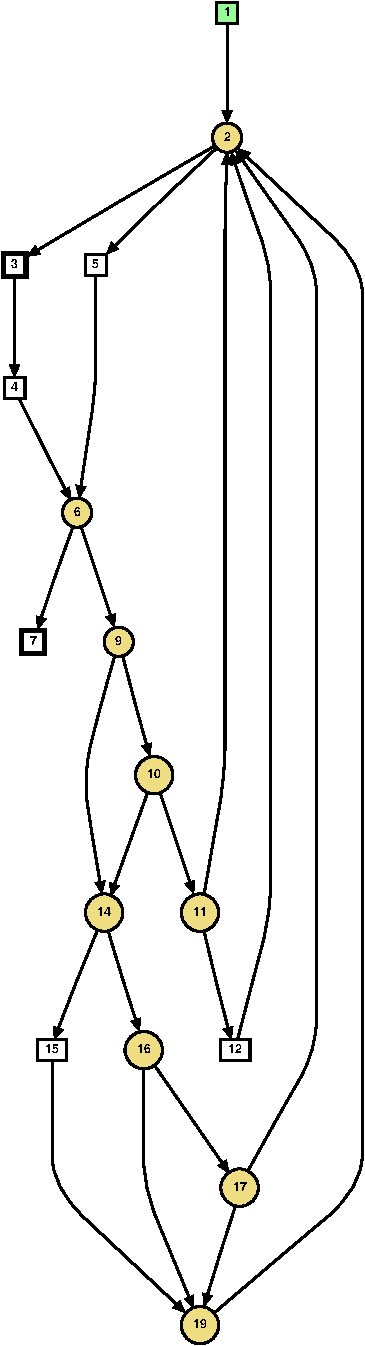
\includegraphics[scale=0.6]{graph1}
    \label{fig:wc1}}
  \subfloat[After if-conversion] {
    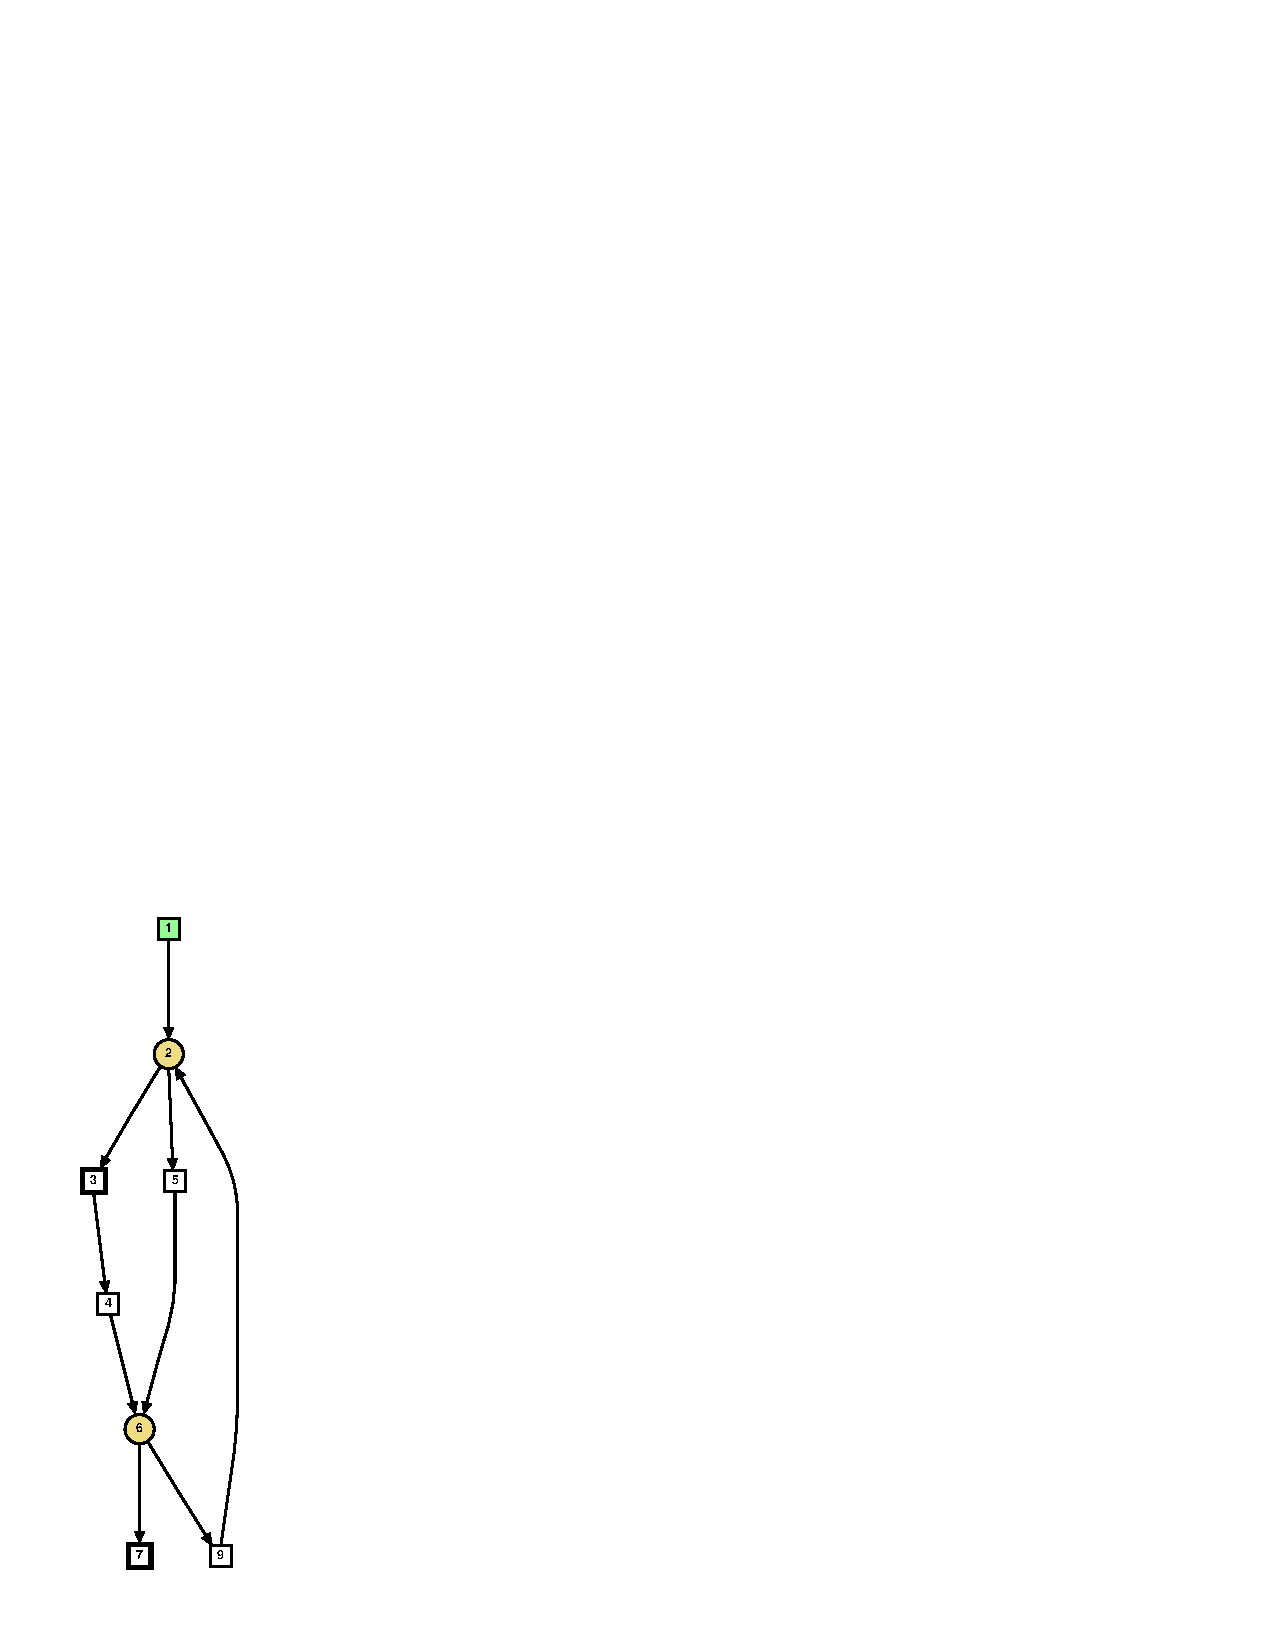
\includegraphics[scale=0.6]{graph7}
    \label{fig:wc2}}
\label{fig:wc example}
\end{figure}

\subsection{Tail Duplication}

Consider the example of Hyperblock formation \ref{fig:hyper1}. This loop contains two branches, and so if-converting it would be profitable. However, block selection has excluded BB2 and has integrated BB5, because heuristics have determined that the schedule of BB5 inside BB4 would be beneficial. The hyperblock contains {BB1, BB3, BB4, BB5, BB6}. Since BB4 has a side entry, it must be removed by tail duplication. \ref{fig:hyper2} shows the control flow after block duplication. Notice that a new node, BB7, has been added after the tail duplication by a process called branch coalescing. Finally \ref{fig:hyper3} shows the code once if-converted.

\begin{figure}[h]
  \subfloat[loop] {
    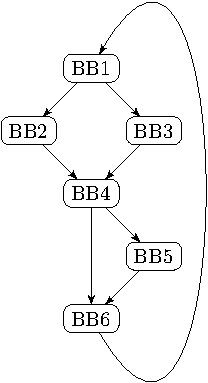
\includegraphics[scale=0.7]{hyper1}
    \label{fig:hyper1}}
  \subfloat[standard tail-duplication] {
    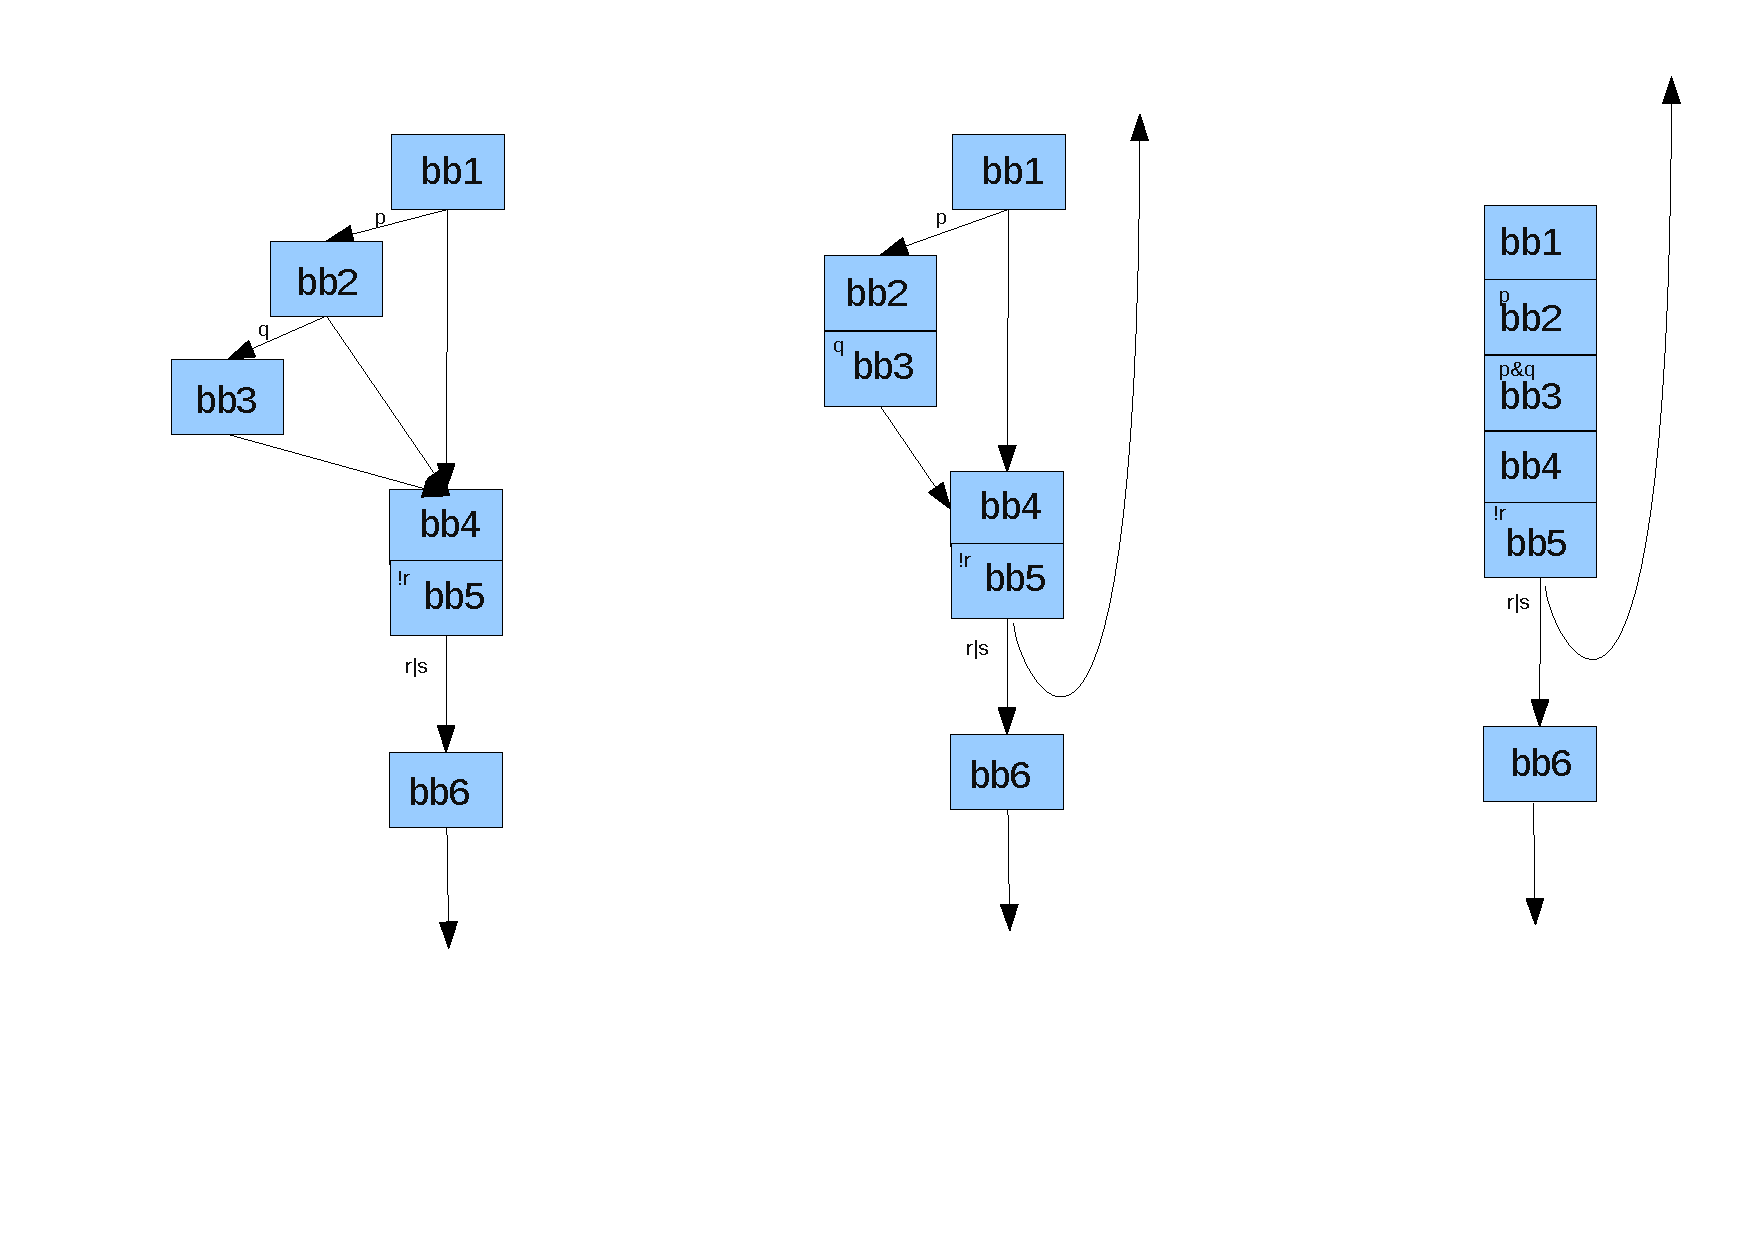
\includegraphics[scale=0.7]{hyper2}
    \label{fig:hyper2}}
  \subfloat[after SSA if-conversion] {
    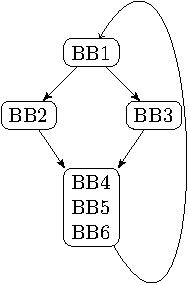
\includegraphics[scale=0.7]{hyper4}
    \label{fig:hyper4}}
  \subfloat[final flow] {
    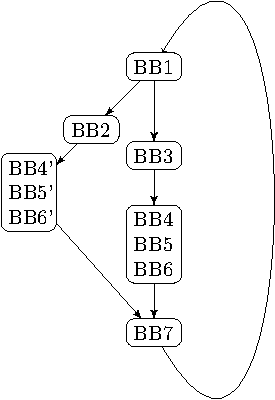
\includegraphics[scale=0.7]{hyper3}
    \label{fig:hyper3}}
\end{figure}

When using this standard decomposition, the if-conversion is performed after tail-duplication. Hyperblock formation, if-conversion and speculation introduce a major phase ordering problem. 

Consider in contrast how tail-duplication can be performed lazily using the SSA iterative transformations, after the code have been if-converted. \ref{fig:hyper4} shows the same loop body where the second $if$ region has been SSA if-converted. The decision to if-convert the region formed by {BB1, BB2, BB3} is now local and can be taken conservatively. Only at this stage, if necessary, tail-duplication can be performed to remove the side entry coming from BB2. Duplicating a single predicated block is now a very simple operation.

\subsection{Profitability}

The objective functions must contain variables not known at the start of the transformation. (such as the complexity of the predicate equations) since moving multiple control flow paths together can easily exceed processors resources (leading to excessive register pressure) or move infrequently used expensive instruction (memory loads) into the critical path. 

The decision to include a basic block into an hyperblock is one of the main difficult trade-off that a good if-conversion algorithm as to deal with. It should be aggressive enough to maximize the use of resources, but without over-committing them, because of the risk of spilling registers or bad schedule if multiple instruction dependent of a scare resource. e.g a multiplier, a data bus or a floating point unit. Lead to conservative heuristics, or reverse if-conversion.

In contrast, the SSA iterative restructuring framework described earlier reduces the scope for the decision function to a very well localized part of the control flow graph. Furthermore, the predicate instructions or temporary register to hold the speculated instructions are already in the code that we are considering. Consequently, SSA iterative if-conversion construction is much more precise. The following factors are considered locally: 

- Semantics. The merge of different execution path should guarantee that the semantics of the program are preserved.
- If-conversion increases register pressure, for two reasons: live ranges are merged and register renaming imposes new constraints
- Schedule length: New data dependencies between a predicate definition and its use, or between a speculated instruction and its merge, can impede the schedule.

Since the execution cannot use dynamic branch prediction schemes to statically schedule the code, it is essential for the compiler to rely on accurate static branch prediction information. Using such information, the block selection process can decide whether the inclusion of one path into the other will be beneficial. 

The first consequence is that all registers are now alive simultaneously, (live range), so the benefits of branch removal and better scheduling is balanced with increased live range and register pressure : If-conversion must rely on an efficient decision model.

The basic idea for decision taking is that a region can be if-converted if the cost of the resulting if-converted basic block is smaller than the cost of each region taken separately weighted by the branch frequencies. The cost is a factor of 2 parameters: resource usage and schedule length.

We compare the pondered cost of the region before if-conversion. So the cost of a path is the schedule estimation of all the blocks in the path pondered by the probability of execution:
\begin{align}
Cost(path)=Freq(path)*\sum_{k=1}^n(Cost(bb_{k}))
\end{align}
The cost of the region starting at basic block $head$ before if-conversion is therefore the cost of all the basic blocks in the considered region, on each path.
\begin{align}
Cost(head)=Cost(bb_{head})+branch\:lat+Cost(taken\:path)+Cost(fall-though\:path)
\end{align}
One of the paths can be empty, in this case only the non empty path will be speculated and it has a zero cost. The Cost after if-conversion is estimated with:
\begin{align}
Cost(head)=Cost(bb_{head} o bb_{taken path} o bb_{fall-though path})
\end{align}

Where $o$ is the composition function that merges basic blocks together, removes associated branches and creates the predicate operations. The resulting $Cost$ applied to the new basic block represents the estimated schedule after if-conversion, that will be effective only if $Cost(head_{before\,ifc}) > Cost(head_{after\,ifc})$. 
 
The cost function uses the target's machine interface information for instruction latencies, resources usage and scheduling constraints to estimate the local scheduling. The local dependencies computed between instructions are used to compute the dependence height. The branch frequency is obtained either from static branch prediction heuristics, profile information or user inserted directives.
\begin{figure}
    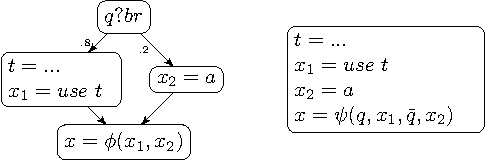
\includegraphics[scale=0.8]{ssa_freq}
\caption{example of profitable if-conversion}
\label{fig:ssa_freq}
\end{figure}

In example \ref{fig:ssa_freq} the dependence height of the fall-through path is 4 cycles. The dependence height of the taken path is 2 cycles. So the estimated cost of the region is 1+2.4+0.2+1=4.6 cycles. The estimated cost of the if-converted region is the schedule height estimation of the instructions without the branches. In this case, 4 cycles. Since the schedule height of the if-converted region is smaller than the profiled estimation, then it is profitable.
It should be noted that this heuristic does not take into account increased register pressure in the case of speculation, because the variables now interfere. Computing the interference graph and simulating a register coalescing process would be extremely expensive at this stage. In the example above, a conservative approach would evaluate a register pressure of 4, without counting than $s$ and $t$ coalesce and that in reality the register budget would be 3. Note that this problem is general to every if-conversion algorithm, but might be more easy to deal with in the SSA framework because of the locality of the region.

\section{Local Transformations}

\subsection{SSA operations on basic blocks}

\begin{figure}[h]
\centering
  \subfloat[phi removal] {
  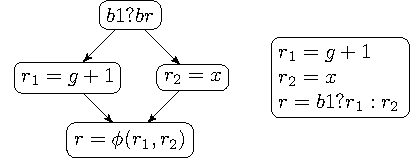
\includegraphics[scale=0.8]{phi_removal}
  \label{fig:phi_rem}}
  \subfloat[phi reduction] {
  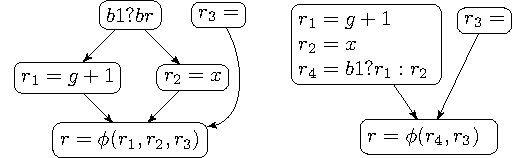
\includegraphics[scale=0.8]{phi_reduction}
  \label{fig:phi_red}}

  \subfloat[phi augmentation] {
  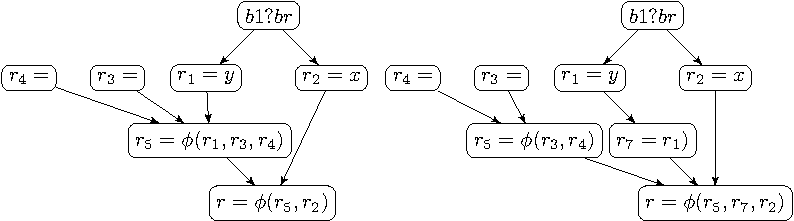
\includegraphics[scale=0.8]{phi_augmentation}
  \label{fig:phi_aug}}
\caption{SSA transformations}
\label{fig: phi_operations}
\end{figure}

The structural if-conversion analysis is based on hammock graphs. A hammock is a single-entry single-exit control flow region $H$ with a distinguished entry node $e$ in $H$ and a distinguished exit node not in $H$. We only need to consider the minimal hammock graph of $H$, which is the smallest hammock sub-graph containing $e$. Any othe nested depth level of hammocks will be optimized by construction.

Structured programming can produce more sophisticated control flows, we describe later restructuring techniques to isolate the candidate region, and remove problematic edges, such as tail duplication, block duplication or conjunctive blocks merging. 

For now we restrict the transformation to the speculative and conditional move model. We use the $select$ like notation $r=c?:r_1:r_2$, to represent the speculative execution of instruction defining $r_1$ and $r_2$. $r$ takes the value of $r_1$ if $c$ is True, else $r_2$. 

Consider a conditional branch depending on a predicate $p$ and a region starting at $BBhead$. Let $BBp$ be the set of single exit basic blocks $(BBi,\dots,BB_n)$ that are on the taken path if $p$ is true and $BBq$ be the set of single exit basic blocks $(BBj,\dots,BB_m)$ that are executed if $p$ is false. The merge point of the if-converted region is at $BBjoin$. We distinguish three types of basic SSA transformations:

\subsubsection{$\phi$ removal} (figure \ref{fig:phi_rem})
The join node of the considered region has two predecessors and the $\phi$ instructions are of the form $r=\phi(r_1,r_2)$. After $r_1$ and $r_2$ speculation the instruction can be rewritten as $r=p?r_1:r_2$.
Once $BBp$ and $BBq$ have been promoted into $BBhead$, $BBjoin$ has $BBhead$ as its unique predecessor, so it is no longer in its dominance frontier. The $\phi$ instruction can then be discarded.

\subsubsection{$\phi$ reduction} (figure \ref{fig:phi_red})
 The join node of the considered region has $n$ predecessors with $\phi$ instructions of the form $r=\phi(r_1,r_i,r_j,\dots,r_n)$. After merging, the $\phi$ operation is rewritten $t=p?r_i,?r_j$. Since $BBjoin$ is still in the dominance frontier of $BBhead$, a new $\phi\:r=\phi(r_1,t,\dots,r_{n-1})$ is redefined with the new defitnitions. The merging instruction is inserted after the speculated $r_i$ and $r_j$ definitions into $BBhead$.
The join block $E$ has $n$ predecessors with $n > 2$, and $n$ blocks in its dominance frontier if it contains $\phi$s.

\subsubsection{$\phi$ augmentation} (figure \ref{fig:phi_aug})
The objective is to remove incoming edges from the hammock. Consider a join side node with $n$ predecessors among which $p$ is duplicated into $q$.  The join node of the considered region have $\phi$ instructions of the form $r=\phi(r_1,p,r_i,r_j,\dots,r_{n-1})$. The instruction is rewritten $t=select(p,r_i,r_j)$ and \mbox{$r=\phi(r_1,t,q,\dots,r_n)$}. 
The duplicated blocks are new dominators of $BBjoin$ that define new $defs$. These blocks are now in the dominance frontier of $BBjoin$. SSA is maintained with new $\phi$ upgraded with the new reaching points.

The newly structure hammock can now in turn by phi reduced. Not shown here, data flow dependencies are broken so new opportunities scalar local optimization arise. Since $r1$ can be propagated into the $\phi$, simplifying the region analysis.


The algorithm to find the predicate value on which each phi operand depends on is straightforward. It is the value for which the successor of $BBhead$ that dominates the basic block defining the phi operand is taken.

\subsubsection{Predicate merging}

During the region formation, subregions containing a block that is reached from two conditions can be optimized by merging predicates. A new predicate is computed using a logical operation on both basic blocks' predicates after a normalization pass. Simple logical operations are usually caught as a peephole or during the instruction selection mechanism, but making it part of the if-conversion process allows it to handle more complex regions because our predicate merging algorithm is not limited to basic blocks that only define predicates, making instructions depending on predicates merge part of the generic SSA speculation framework. However, this transformation is very sensitive to biased branches since each conditional operation now depends on two predicates instead of one that cannot be scheduled together because of the computation of the logical operation making it more difficult to compensate for the branch removal. In order to avoid long sequences data dependencies and break schedule, we exclude from this promotion predicates that depend on long latency operations.
Because of new data dependencies introduced by the new computed predicate the performance contribution of this transformation mainly comes from the branch removal (two conditional branches and two direct branches are removed from an if-converted region whose predicates have been merged) rather than local ILP. Predicate promotion and merge is more effective in loop nest regions where more optimizations may extract ILP from it, for example modulo scheduling can extract ILP from such if-converted bodies by overlapping different iterations. 

*note: rework. Explain cunjunctive branch optimisation*
We allow two successive conditional blocks sharing one immediate post-dominator to be merged with logical operations after a normalization transformation. The normalization transformation ensures that conditional blocks sharing a common target can be merged by defining a wired $or$, or a wired $and$ share the same branch characteristics using branch reordering, test inversion or $de-Morgan$ transformations.

\begin{figure}
  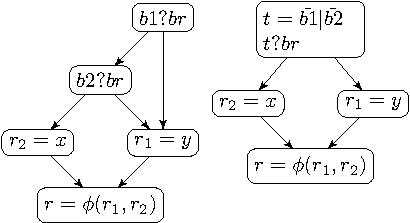
\includegraphics[scale=0.8]{phi_merge}
  \label{fig:phi_merge}
\caption{Predicate merging}
\end{figure}

\subsection{SSA representation of conditional instructions}

One problem of the described SSA-speculative framework is that it does not fit very well with a predicated model of conditional execution. Since $\phi$ instructions are transformed to turn joint points into conditional moves, we should backtrack to transform conditional moves into predicated instructions. This process of transforming speculation into predication is not convenient for many reasons:
- Predicated instructions introduce a renaming problem: A same register name can have two different assignments (under different predicates), which breaks the SSA property of single static assignment. The solution is to re-use the framework that converts join points into an extended SSA representation:

In the $\psi$-SSA representation, the edge dependency from the basic block into which the definition of the $\phi$ argument is defined in the original CFG is replaced by a new data dependency. This dependency needs to be materialized into a $select$ or $\psi$ operation. Note that the $select$ operation is a real instruction that does not need to be replaced during the out-of-SSA phase. If the target architecture does not provide such instruction to switch between speculated instruction, it can be emulated using two conditional moves. One advantage to generate $select$ instruction at this stage is that the program stays in full SSA form and make all the data dependencies explicit, and can be feed to all SSA optimizers. 

\begin{figure}
\begin{minipage}[t]{3.5cm}
\mbox{SSA:} \\
$ if (p) $ \\
$   x_1 = a+b $ \\
$ else $ \\
$   x_2 = 0 $ \\
$ x = \phi (x_1, x_2) $ \\
\end{minipage}
\begin{minipage}[t]{3.5cm}
\mbox{SSA-speculative form:} \\
$x_1 = a + b $ \\
$x_2 = 0 $ \\
$x = p \cond  x_1 : x_2$ \\
\end{minipage}
\begin{minipage}[t]{3.5cm}
\mbox{$\psi$-SSA form:} \\
$x_1 = a + b $ \\
$x_2 = 0 $\\
$x = \psi (p \cond x_1, \overline{p} x_2) $ \\
\end{minipage}
\end{figure}

Note that unlike $\phi$ arguments that are executed simultaneously (they don't depend each other), $\psi$ arguments are executed sequentially and ordered from their definition predicate set. This property is necessary because of the new data dependencies introduced into the straight line of predicated code stream.

The basic idea behind the SSA transformations is to replace $\phi$ operations by predicated instructions merging into a $\psi$ or speculated instructions merging into a $select$ equivalent instruction, while maintaining the SSA properties.

\subsection{SSA promotion}

In SSA form, we distinguish two kind of speculative execution. Unconditional speculation is the speculation of an instruction whose the result operand does not appear has a $\phi$ operand, it can be emitted has such. Conditional speculation is the execution of an instruction whose the result merge into a $\phi$ operand inside the hammock. Such result will need to be conditionalize and a data dependency with the predicated created.

To identify the operation's results that need to be conditionally defined, we only need to look at the defining instructions of the $\phi$ instructions. By elimination, all temporaries that do not have a join point into the considered region and that don't have a side effect can be unconditionally speculated during the SSA transformations processes. Only instructions with a side effect need to be guarded. This is a considerable advantage over traditional if-conversion algorithms that marks all instructions in a conditional basic block as dependent on the predicate. By removing this predicate dependency, which is a data dependency, the instruction can be moved before the predicate assignment.

The process is applied iteratively on the CFG in SSA form until no more reductions are possible. The quality of the SSA taken as input does not affect the correctness of the algorithm: if the control flow is in pruned SSA, i.e two paths $x->+z$ and $y->+z$ converge at node z, then a $\phi$ node is inserted at z only if z is alive in or after z. in which case x and y are promoted and no $select$ operation is generated. If the SSA is minimal, a $select$ instruction would be generated and removed by dead code. Inserting dead code from minimal SSA only introduces noise in the local scheduling heuristics because of the false data dependencies.

\subsubsection{Partial redefinition}

A $\psi$ operation exposes new data dependencies, by expressing the merge of two definitions. Note that the order of the partial definition is important, because a definition partially redefines the preceding ones. We use this property to speculate the first definitions, so it becomes speculated instead of disjoint. This local optimization allows the removal of predicate dependency but also creates a new partial dependency when predicates are not disjoint. 

\begin{figure}
\footnotesize
\begin{minipage}[t]{4cm}
\mbox{disjoint predicates} \\
$ p = test $ \\
$ p \cond x_1 = a + b $ \\
$ \overline{p} \cond x_2 = c $ \\
(1) $ x = \psi(p \cond x_1, \overline{p} \cond x_2) $ \\
\end{minipage}
\begin{minipage}[t]{4cm}
\mbox{optimized order predicates} \\
$ x_1 = a + b $ \\
$ p = test $ \\
$ \overline{p} \cond x_2 = c $ \\
$ x = \psi(T \cond x_1, \overline{p} \cond x_2) $ \\
\end{minipage}
\end{figure}

$T$ represents the $True$ predicate. This optimization is useful to save one predicate register and to remove a data dependency between a predicate definition and its use. 
The $\psi$ definition is defined on the $T$ predicate set, therefore it is speculable, as shown below:

\subsubsection{$\psi$ speculation properties}

Since $\psi$ operations are part of the intermediate representation, they can be considered for inclusion in a candidate region for if-conversion. The conditional operations that the refer can be in turn speculated or predicated iteratively. We define here the promotion rules for $\psi$ operands, whereas the instructions defining the $\psi$ operands will be speculated.

Consider the instructions \ref{nested_psi} containing a subregion already processed. The $\psi$ operation can be safely speculated if all the instructions defining its operands can be speculated: they don't produce hazardous execution, they don't produce any side effects and there exists a conditional move instruction to merge the operands. Then the block can be executed regardless of the value of $c$. The use of the $\psi$ result is also unconditionally executed.

\subsubsection{$\psi$ predication properties}

If an instructions is not speculable, it must be predicated:
In \ref{nested_psi_predicated}, the $c$ condition merges with all conditions under which the $\psi$ operands are defined. Here a new predicate $p_1$ is created to hold the predicate definition for the instructions defined under $c$. 

Note that conceptually, the speculative $\psi$ execution allows a predicate definition domain larger that the original one, which the predicative transformation exactly matches the initial definition domain, at the expense of more data dependencies and predicate computation.

We can see with this example that the decision to speculate or predicate can be done at the level of each joining definition, allowing a mix of them in the final program. The advantage to speculation over predication is a reduced dependency length. The disadvantage of speculation is that it increases register pressure until the merge point, and puts long latency operations on the critical path.
 
\begin{figure}
\footnotesize
\begin{minipage}[t]{3.5cm}
\mbox{nested if} \\
$ if (c) $ \\
$ \{ $ \\
\hspace*{2mm}$ x_1 = a + b $ \\
\hspace*{2mm}$ \overline{p} \cond x_2 = c $ \\
\hspace*{2mm}$ x = \psi(T \cond x_1, \overline{p} \cond x_2) $ \\
\hspace*{2mm}$ d_1 = use (x) $ \\
$ \} $ \\
$ else $ \\
\hspace*{2mm}$ d_2 = 3 $ \\
$ d = \phi(d_1,d_2) $ \\
\label{nested_psi}
\end{minipage}
\begin{minipage}[t]{3.5cm}
\mbox{speculated nested} \\
$ x_1 = a + b $ \\
$ \overline{p} \cond x_2 = c $ \\
$ x = \psi(T \cond x_1, \overline{p} \cond x_2) $ \\
$ d_1 = use (x) $ \\
$ \overline{c} \cond d_2 = 3 $ \\
$ d = \psi(T \cond d_1, \overline{c} \cond d_2) $ \\
\label{nested_psi_speculated}
\end{minipage}
\begin{minipage}[t]{3.5cm}
\mbox{predicated nested} \\
$ p_1 = \overline{p} \& {c} $ \\
$ c \cond x_1 = a + b $ \\
$ p_1 \cond x_2 = c $ \\
$ x = \psi(c \cond x_1, p_1 \cond x_2) $ \\
$ d_1 = use (x) $ \\
$ \overline{c} \cond d_2 = 3 $ \\
$ d = \psi(T \cond d_1, \overline{c} \cond d_2) $ \\
\label{nested_psi_predicated}
\end{minipage}
\caption{Inner region $\psi$}
\end{figure}


\subsubsection{Block duplication}

Block duplication is used to remove side entries and to obviate the constraints on control dependencies. Unless applied carefully, block duplication could be the cause of code bloating without performance improvement. However experience has shown that when applied carefully it can be efficient.
Consider for example in the figure \ref{fig:bbdup}. Since we are if-converting from the inner most regions, the algorithm first considers the region {BB3,BB4,BB5,BB6,BB7}, and discards the edge coming from BB2 by duplicating BB6 into BB8. The $\phi$ becomes a move in the duplicated block with a renamed definition. The new $\phi$ operands are updated from the new edge. Note that in the implementation the block does not need to be created since it will be next promoted into BB3. We have two nested hammocks and the process can iterate. The dependency that has been removed in the control flow is now expressed as a data dependency between the two $select$ instructions.

The algorithm to perform SSA block duplication is decomposed into:
\begin{itemize}
\item Extract the $\phi$s definitions to be conditionalized from the duplicated block creating a $move$ instruction and a new reduced $\phi$ (or two $move$ instructions if the duplicated block had only two incoming edges).
\item Then the $\phi$s in the tail basic block are augmented with the new def created by the new repair instruction. If the $\phi$ was live-out after the tail block a move must be inserted to avoid propagating renaming outside of the region considered. 
\item The last step consists of renaming the new definitions to keep the region in SSA form.
\end{itemize}

\begin{figure}[h]
\centering
  \subfloat[Original] {
    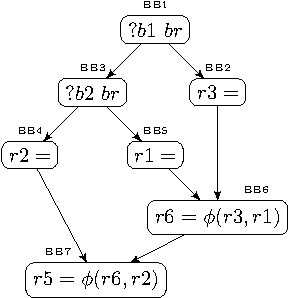
\includegraphics[scale=0.75]{side1}
    \label{fig:side1}}
  \subfloat[After duplication] {
    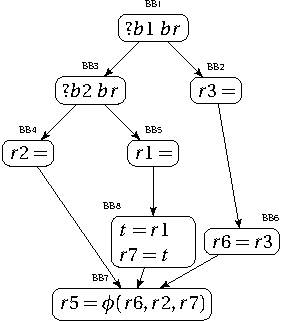
\includegraphics[scale=0.75]{side2}
    \label{fig:side2}}
  \subfloat[sub-region 1] {
    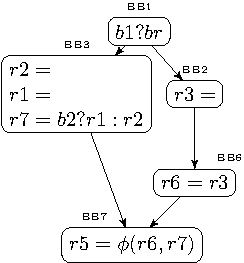
\includegraphics[scale=0.75]{side3}
    \label{fig:side3}}
  \subfloat[sub-region 2] {
    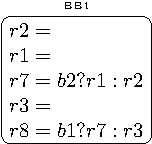
\includegraphics[scale=0.75]{side4}
    \label{fig:side4}}
\caption{Side entry removal using block duplication}
\label{fig:bbdup}
\end{figure}


\section{Conclusion} 
We presented in this chapter how an if-conversion algorithm can take advantage of the SSA properties to efficiently assign predicates and lay out the new control flow in an iterative, inner-out process. As opposed to the other top-down approach, the region selection can be reevaluated at each nested transformation, using local analysis.
Basic block selection and if-conversion are performed as a single process, hyperblocks being created lazily, using well known techniques such as tail-duplication or branch coalescing only when the benefit is established.
Predication and speculation are often presented as two different alternatives for if-conversion. While it is true than they both require different hardware support, they should coexist in an efficient if-conversion process so every model of conditional execution is accepted. Thanks to conditional moves and $\psi$ transformations, they are now generated together in the same framework.

\section{Additional reading}

In its cornerstone work, \cite{Rau:2003:IP:1074100.1074489}, exposes ILP in VLIW architectures using trace scheduling and local if-converted if-then-else regions using the $select$ and dismissible load operations. The idea behind was to let to the compiler the bulk to statically reorganize the instruction. In this respect, predictability \cite{Fisher:1992:PCB:143371.143493} becomes a major criteria for profitability.

With hard to predict profitability in conventional if-conversion algorithms, Reverse if-conversion \cite{August:1999:PRI:326224.325595} was proposed, reconstructing the control flow at schedule time, after applied more aggressive region selection criteria.
Hyperblocks \cite{Mahlke:1992:ECS:144965.144998} was proposed as the primary if-converted scheduling framework, excluding basic blocks that does not justify their inclusion into the if-converted flow of control.

The duality between SSA like $\phi$s and predicate dependencies have been used in other works. In SSA-PS \cite{Jacome01clusteredvliw}, Predicated Switching operations are used to realize the conditional assignments using aggressive speculation techniques with conditional moves. Phi-Predication \cite{Chuang03phi-predicationfor} uses a modified version of the RK algorithm, to map phi-predication with phi-lists, holding guard and topological information. In both works, the use of SSA like aims at solving the multiple definition problem exploiting variable renaming and join points, but they are based on speculation using conditional moves. 

In \cite{Stoutchinin_Gao_2004}, $\psi$ instructions are inserted while in SSA using a modified version of the classical Fang algorithm \cite{Fang:1996:CAI:645674.663446}, enabling the support for a fully predicated ISA.
Those work established that standard if-conversion techniques can be applied to a SSA form using the $\psi$-SSA representation, or light weight $\phi$-SSA generation, but does not yet exploit the native SSA properties to build up the if-converted region.
A global SSA framework was presented \cite{odes_bruel} to support $select$ moves using aggressive speculation techniques, further extended to $\psi$-SSA \cite{ijes_bruel} allowing a mix of speculative and predicated techniques.

If-conversion was studied to be very effective on embedded processors to sustain performance in loop intensive computation required for multimedia applications \cite{FisherFaraboshiYoung}. In the mathematical for evaluation of polynomial expressions \cite{Jeannerod:2010:TTI:1837210.1837212} allowing the generation of straight line code, despite the presence of exit tests in the algorithm allowing aggressive schedules.




